\documentclass[handout]{beamer}
\usepackage[utf8]{inputenc}
\usepackage[english]{babel}
\usepackage{helvet}
\usepackage[T1]{fontenc}
\usepackage{textcomp}
\usepackage[inline]{asymptote}
\usepackage{slide_helper}
\usepackage{tikz}
\usetikzlibrary{shapes.geometric, arrows}
\usepackage{pgfplots}
\pgfplotsset{compat=1.5} 
\usepgfplotslibrary{statistics}
\usetikzlibrary{external}
\tikzexternalize%

\title[MA205 - Section 2.1]{Examining Numerical Data}

\begin{document}
\begin{frame}
\titlepage
\end{frame}

\begin{frame}
\begin{example}
Let us consider a scatterplot of borrowers total income and the loan amount from the \texttt{loan50} data set.

\only<1| handout:0>{
\begin{center}
\begin{tikzpicture}
\tikzstyle{every pin}=[
fill=white,
draw=black,
font=\tiny,
]
\pgfkeys{/pgf/number format/.cd,
fixed,
precision=999,
set thousands separator={},
1000 sep in fractionals=false,
}
\begin{axis}[
clip mode=individual,
clip marker paths=true,
width=11.5cm,
height=5cm,
xlabel={Total Income},
ylabel={Loan Amount},
grid=major,
%ymajorgrids=true,
%xmajorgrids=true,
%enlarge x limits=false,
%enlarge y limits=false,
%xticklabel style={/pgf/number format/.cd,fixed,precision=0},
xticklabel=\$\pgfmathprintnumber{\tick}k,,
yticklabel=\$\pgfmathprintnumber{\tick}k,,
xtick={0, 50000, 100000, 150000, 200000, 250000, 300000},
ytick={0, 10000, 20000, 30000, 40000},
scaled x ticks=base 10:-3,
xtick scale label code/.code={},
scaled y ticks=base 10:-3,
ytick scale label code/.code={},
ymin=-5,
ymax=35000,
xmin=-5,
xmax=325000,
scatter/use mapped color={
%draw=mapped color,
fill=black,
},
]
\addplot [scatter, only marks, blue!50!black, scatter src=y, mark size=0.8pt] 
table [y=loan_amount, x=total_income, col sep=comma] {loan50.csv};
\end{axis}
\end{tikzpicture}
\end{center}
}
\only<2->{
\begin{center}
\begin{tikzpicture}
\tikzstyle{every pin}=[
fill=white,
draw=black,
font=\tiny,
]
\pgfkeys{/pgf/number format/.cd,
fixed,
precision=999,
set thousands separator={},
1000 sep in fractionals=false,
}
\begin{axis}[
clip mode=individual,
clip marker paths=true,
width=11.5cm,
height=5cm,
xlabel={Total Income},
ylabel={Loan Amount},
grid=major,
%ymajorgrids=true,
%xmajorgrids=true,
%enlarge x limits=false,
%enlarge y limits=false,
%xticklabel style={/pgf/number format/.cd,fixed,precision=0},
xticklabel=\$\pgfmathprintnumber{\tick}k,,
yticklabel=\$\pgfmathprintnumber{\tick}k,,
xtick={0, 50000, 100000, 150000, 200000, 250000, 300000},
ytick={0, 10000, 20000, 30000, 40000},
scaled x ticks=base 10:-3,
xtick scale label code/.code={},
scaled y ticks=base 10:-3,
ytick scale label code/.code={},
ymin=-5,
ymax=35000,
xmin=-5,
xmax=325000,
scatter/use mapped color={
%draw=mapped color,
fill=black,
},
]
\addplot [scatter, only marks, red, scatter src=y, mark size=1.0pt, scatter/use mapped color={fill=red,}]
table [y=loan_amount, x=total_income, col sep=comma, x expr={\thisrow{total_income} / (\thisrow{total_income} <= 100000)}] {loan50.csv};
\addplot [scatter, only marks, blue!50!black, scatter src=y, mark size=0.8pt]
table [y=loan_amount, x=total_income, col sep=comma, x expr={\thisrow{total_income} / (\thisrow{total_income} > 100000)}] {loan50.csv};
\addplot [mark size=0pt, red, line width=0.5pt] coordinates {(100000,0) (100000,35000)};
\end{axis}
\end{tikzpicture}
\end{center}
}\pause

We can see that the many of borrowers earn \$100,000 a year or less.
\end{example}
\end{frame}

\begin{frame}
\begin{example}
Let us consider a scatterplot of borrowers total income and the loan amount from the \texttt{loan50} data set.

\only<1| handout:0>{
\begin{center}
\begin{tikzpicture}
\tikzstyle{every pin}=[
fill=white,
draw=black,
font=\tiny,
]
\pgfkeys{/pgf/number format/.cd,
fixed,
precision=999,
set thousands separator={},
1000 sep in fractionals=false,
}
\begin{axis}[
clip mode=individual,
clip marker paths=true,
width=11cm,
height=5cm,
xlabel={Poverty Rate},
ylabel={Median Household Income},
grid=major,
%ymajorgrids=true,
%xmajorgrids=true,
%enlarge x limits=false,
%enlarge y limits=false,
%xticklabel style={/pgf/number format/.cd,fixed,precision=0},
xticklabel=\pgfmathprintnumber{\tick}\%,
yticklabel=\$\pgfmathprintnumber{\tick}k,
xtick={0, 10, 20, 30, 40, 50},
ytick={0, 20000, 40000, 60000, 80000, 100000, 120000},
%scaled x ticks=base 10:-3,
%xtick scale label code/.code={},
scaled y ticks=base 10:-3,
ytick scale label code/.code={},
ymin=-5,
ymax=125000,
xmin=-5,
xmax=60,
scatter/use mapped color={
%draw=mapped color,
fill=black,
},
]
\addplot [scatter, only marks, blue!50!black, scatter src=y, mark size=0.3pt] 
table [y=median_hh_income, x=poverty, col sep=comma,ignore chars={N,A}] {county.csv};
\end{axis}
\end{tikzpicture}
\end{center}
}
\only<2->{
\begin{center}
\begin{tikzpicture}
\tikzstyle{every pin}=[
fill=white,
draw=black,
font=\tiny,
]
\pgfkeys{/pgf/number format/.cd,
fixed,
precision=999,
set thousands separator={},
1000 sep in fractionals=false,
}
\begin{axis}[
clip mode=individual,
clip marker paths=true,
width=11cm,
height=5cm,
xlabel={Poverty Rate},
ylabel={Median Household Income},
grid=major,
%ymajorgrids=true,
%xmajorgrids=true,
%enlarge x limits=false,
%enlarge y limits=false,
%xticklabel style={/pgf/number format/.cd,fixed,precision=0},
xticklabel=\pgfmathprintnumber{\tick}\%,
yticklabel=\$\pgfmathprintnumber{\tick}k,
xtick={0, 10, 20, 30, 40, 50},
ytick={0, 20000, 40000, 60000, 80000, 100000, 120000},
%scaled x ticks=base 10:-3,
%xtick scale label code/.code={},
scaled y ticks=base 10:-3,
ytick scale label code/.code={},
ymin=-5,
ymax=125000,
xmin=-5,
xmax=60,
scatter/use mapped color={
%draw=mapped color,
fill=black,
},
]
\addplot [scatter, only marks, blue!50!black, scatter src=y, mark size=0.3pt] 
table [y=median_hh_income, x=poverty, col sep=comma,ignore chars={N,A}] {county.csv};
\addplot [domain=0:50,red, line width=1pt] {84923*e^(-0.0342*x)};
\end{axis}
\end{tikzpicture}
\end{center}
}\pause
It is clear there is a \textbf{nonlinear} association between the median household income and the poverty rate.
\end{example}
\end{frame}

\begin{frame}
\begin{definition}
A \textbf{dot plot} is a one-variable scatterplot. Each data value is plotted as a point above a horizontal scale of values. Dots representing equal values are stacked.
\end{definition}\pause

\begin{note}
Dot plots work best with integer data. It is common to round decimals before building a dot plot.
\end{note}\pause

\begin{example}
\begin{center}
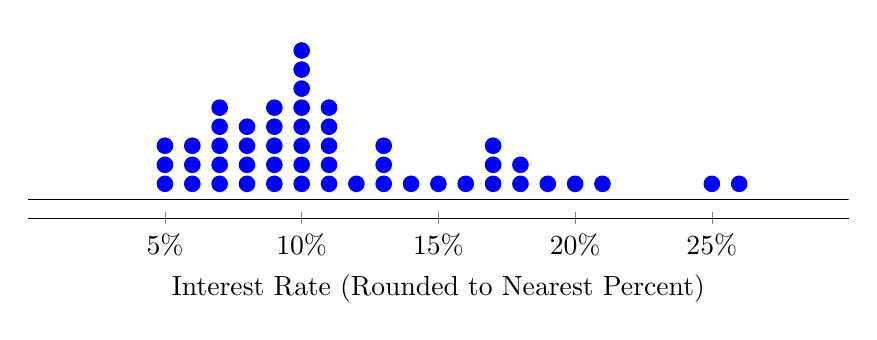
\begin{tikzpicture}
\pgfplotsset{ every non boxed x axis/.append style={x axis line style=-},
     every non boxed y axis/.append style={y axis line style=-}}
\begin{axis}[
width=12cm,
height=4cm,
xlabel={Interest Rate (Rounded to Nearest Percent)},
ylabel={},
yticklabels={},
axis y line=none,
axis x line=bottom,
xticklabel=\pgfmathprintnumber{\tick}\%,
xtick={5,10,15,20,25},
ymin=0,
ymax=10,
xmin=0,
xmax=30,
scatter/use mapped color={
 %draw=mapped color,
 fill=blue,
},
]
\addplot[domain=0:30]  {1};
\addplot[scatter, only marks, blue, scatter src=y, mark size=2.8pt]
coordinates
{
(11, 1.8)
(11, 2.8)
(11, 3.8)
(11, 4.8)
(11, 5.8)
(10, 1.8)
(10, 2.8)
(10, 3.8)
(10, 4.8)
(10, 5.8)
(10, 6.8)
(10, 7.8)
(10, 8.8)
(26, 1.8)
(9, 1.8)
(9, 2.8)
(9, 3.8)
(9, 4.8)
(9, 5.8)
(17, 1.8)
(17, 2.8)
(17, 3.8)
(6, 1.8)
(6, 2.8)
(6, 3.8)
(8, 1.8)
(8, 2.8)
(8, 3.8)
(8, 4.8)
(13, 1.8)
(13, 2.8)
(13, 3.8)
(5, 1.8)
(5, 2.8)
(5, 3.8)
(7, 1.8)
(7, 2.8)
(7, 3.8)
(7, 4.8)
(7, 5.8)
(25, 1.8)
(18, 1.8)
(18, 2.8)
(19, 1.8)
(14, 1.8)
(20, 1.8)
(15, 1.8)
(12, 1.8)
(16, 1.8)
(21, 1.8)
};
\end{axis}
\end{tikzpicture}
\end{center}
\end{example}
\end{frame}

\begin{frame}
\begin{definition}
A \textbf{parameter} is a numerical measurement describing some characteristic of a population.
\end{definition}\pause
\begin{definition}
A \textbf{statistic} is a numerical measurement describing some characteristic of a sample.
\end{definition}\pause
\begin{note}
Parameter and population both start with a \textquote{P.}\\Statistic and sample both start with a \textquote{S.}
\end{note}
\end{frame}

\begin{frame}
\begin{definition}
A \textbf{measure of center} is a value at the center or middle of a data set.
\end{definition}\pause

\begin{definition}
The \textbf{mean} of a set of data is the measure of center found by adding all the data values and dividing by the total number of data values.
\end{definition}\pause

\begin{note}
The mean is also known as the \textbf{average}.
\end{note}\pause

\begin{block}{Properties of the Mean}
\begin{itemize}
\item Sample means drawn from the same population tend to vary less than other measures of center.\pause
\item A disadvantage of the mean is that just one extreme value can change the value of the mean substantially.
\end{itemize}
\end{block}
\end{frame}

\begin{frame}
\begin{block}{Common Notation}
Sample statistics are usually represented by English letters, such as $\bar{x}$, while population parameters are usually represented by Greek letters, such as $\mu$.\pause
\vspace{-4mm}
{\renewcommand*{\arraystretch}{2.2}
\begin{equation*}
\begin{matrix}[ll]
\sum & \text{denotes the sum of a set of data values.} \\\pause
x & \text{is used as a placeholder for the variable of interest.} \\\pause
n & \text{represents the number of data values in a sample.} \\\pause
N & \text{represents the number of data values in a population.} \\\pause
\bar{x}=\dfrac{\sum x}{n} & \text{is the mean of a set of sample values.} \\\pause
\mu = \dfrac{\sum x}{N} & \text{is the mean of all values in a population.}
\end{matrix}
\end{equation*}}
\end{block}
\end{frame}

\begin{frame}
\begin{example}\label{verizon}
Suppose we measure the of data speeds of smartphones from the four major carriers. The table contains five data speeds, in megabits per second (Mbps), from this data set.

\begin{center}
\begin{tabular}{|l|ccccc|}\hline
\text{Carrier} & \text{Verizon} & \text{Verizon} & \text{Verizon} & \text{Verizon} & \text{Verizon}\\
\text{Mbps} & 38.5 & 55.6 & 22.4 & 14.1 & 23.1\\\hline
\end{tabular}
\end{center}\pause

The mean is 
\begin{equation*}
\bar{x} = \dfrac{\sum x}{n}\pause
= \dfrac{38.5 + 55.6 + 22.4 + 14.1 + 23.1}{5}\pause
= \dfrac{153.7}{5}\pause
 = 30.74~\text{Mbps}
\end{equation*}
\end{example}\pause

\begin{note}
Round statistics and parameters to one more decimal place than found in the data.
\end{note}
\end{frame}

\begin{frame}
\begin{note}
It is common to mark the mean on a dot plot.
\end{note}\pause

\begin{example}\label{mean_dotplot}
The mean of \texttt{interest\_rate} is: (Do not round the data values.)
\begin{equation*}
\bar{x}=
\dfrac{\tiny\left(\begin{array}{c}5.31\%+5.31\%+5.32\%+6.08\%+6.08\%+6.08\%+6.71\%+6.71\%+7.34\%\\+7.35\%+7.35\%+7.96\%+7.96\%+7.96\%+7.97\%+9.43\%+9.43\%+9.44\%\\+9.44\%+9.44\%+9.92\%+9.92\%+9.92\%+9.92\%+9.93\%+9.93\%+10.42\%\\+10.42\%+10.9\%+10.9\%+10.91\%+10.91\%+10.91\%+11.98\%+12.62\%\\+12.62\%+12.62\%+14.08\%+15.04\%+16.02\%+17.09\%+17.09\%+17.09\%\\+18.06\%+18.45\%+19.42\%+20\%+21.45\%+24.85\%+26.3\%\end{array}\right)}{50}=11.567\%
\end{equation*}\pause
\vspace{-6mm}
\begin{center}
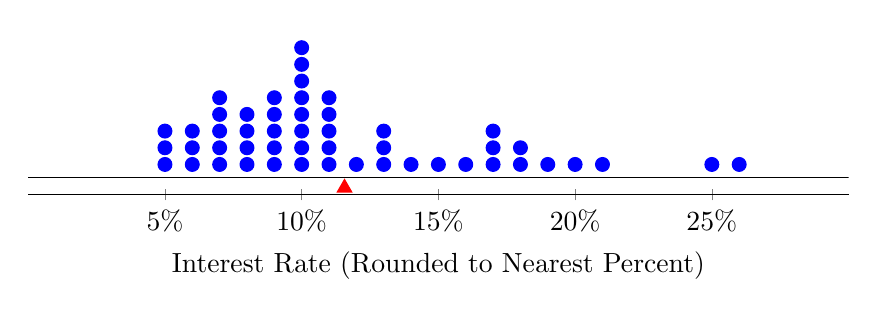
\begin{tikzpicture}
\pgfplotsset{ every non boxed x axis/.append style={x axis line style=-},
     every non boxed y axis/.append style={y axis line style=-}}
\begin{axis}[
width=12cm,
height=3.7cm,
xlabel={Interest Rate (Rounded to Nearest Percent)},
ylabel={},
yticklabels={},
axis y line=none,
axis x line=bottom,
xticklabel=\pgfmathprintnumber{\tick}\%,
xtick={5,10,15,20,25},
ymin=0,
ymax=10,
xmin=0,
xmax=30,
scatter/use mapped color={
 %draw=mapped color,
 fill=blue,
},
]
\addplot[domain=0:30]  {1};
\addplot[scatter, only marks, blue, scatter src=y, mark size=2.5pt]
coordinates
{
(11, 1.8)
(11, 2.8)
(11, 3.8)
(11, 4.8)
(11, 5.8)
(10, 1.8)
(10, 2.8)
(10, 3.8)
(10, 4.8)
(10, 5.8)
(10, 6.8)
(10, 7.8)
(10, 8.8)
(26, 1.8)
(9, 1.8)
(9, 2.8)
(9, 3.8)
(9, 4.8)
(9, 5.8)
(17, 1.8)
(17, 2.8)
(17, 3.8)
(6, 1.8)
(6, 2.8)
(6, 3.8)
(8, 1.8)
(8, 2.8)
(8, 3.8)
(8, 4.8)
(13, 1.8)
(13, 2.8)
(13, 3.8)
(5, 1.8)
(5, 2.8)
(5, 3.8)
(7, 1.8)
(7, 2.8)
(7, 3.8)
(7, 4.8)
(7, 5.8)
(25, 1.8)
(18, 1.8)
(18, 2.8)
(19, 1.8)
(14, 1.8)
(20, 1.8)
(15, 1.8)
(12, 1.8)
(16, 1.8)
(21, 1.8)
};
\addplot [scatter, only marks, red, scatter src=y, mark size=3pt, scatter/use mapped color={fill=red,}, mark=triangle*] coordinates {(11.567, 0.4)};
\end{axis}
\end{tikzpicture}
\end{center}
\end{example}
\end{frame}

\begin{frame}
\begin{example}
We saw in Example~\ref{mean_dotplot} that the average loan interest rate was 11.567\%.

\vspace{1mm}
\question{What is the mean of \textbf{all} loans in the country?}\pause
\answer{The best guess we can make is to use the sample mean of 11.567\%.}\pause

\vspace{2mm}
\question{Is this a good guess?}\pause
\answer{Just because the sample mean is the only educated guess we can make, doesn't mean it's anywhere close to the population mean.}
\end{example}\pause

\begin{definition}
A \textbf{point estimate} is a single value used to estimate a population parameter.
\end{definition}\pause

\begin{note}
We will discuss tools in Chapter 5 and beyond to determine how well a point estimate estimates a parameter.
\end{note}
\end{frame}

\begin{frame}
\begin{example}
We would like to determine if a new drug is more effective at treating asthma attacks than the standard drug. A trial of 1500 adults is setup, giving the following data.

\vspace{-5mm}
\begin{center}
\begin{tabular}{c|cc}
& New drug & Standard drug \\\hline
Number of patients & 500 & 1000 \\
Total asthma attacks & 200 & 300
\end{tabular}
\end{center}
\question{Can we conclude that the new drug is more effective?}\pause
\answer{Raw numbers can be deceptive when group sizes are unbalanced.}\pause
 
 \vspace{1mm}
Looking at the table, 200 is a smaller number than 300. \pause

\vspace{1mm}
But, when we calculate the means we get:

\vspace{-4mm}
\begin{center}
\begin{tabular}{lc}
New drug: & $200~\text{attacks} / 500~\text{patients}=0.4~\text{attacks per patient}$ \\[2mm]
Standard drug: & $300~\text{attacks} / 1000~\text{patients}=0.3~\text{attacks per patient}$
\end{tabular}
\end{center}\pause
The average number of asthma attacks per patient is higher with the new drug, so it's not more effective.
\end{example}
\end{frame}

\begin{frame}
\begin{example}
Emilio opened a food truck last year, and his business has stabilized over the last three months. During this three month period he made $\$11,000$, while working 625 hours.

\vspace{1mm}
\question{Is Emilo doing well with his new business?}\pause
\answer{If you haven't ran a food truck, it can be hard to tell if $\$11,000$ is a high amount or a low amount.}\pause

\vspace{1mm}
Calculating the mean gives:
\begin{equation*}
\dfrac{\$11000}{625~\text{hours}} = \$17.60~\text{per hour}
\end{equation*}
\end{example}\pause

\begin{note}
The mean gives a standardized a metric into something easier to interpret and compare.
\end{note}
\end{frame}

\begin{frame}
\begin{example}
Suppose we want to find the average income per person across the entire United States. To do so, we take the mean of the \texttt{per\_capita\_income} variable from the \texttt{county} data set.

\vspace{1mm}
\question{Is this the best approach?}\pause
\answer{No. Each county represents multiple people. If we computed the mean of \texttt{per\_capita\_income} we  would be treating a county with $5,000$ residents and a county with $5,000,000$ residents the same.}\pause

\vspace{1mm}
To account to differences in the population of each county, we should:
\begin{enumerate}
\item Calculate the total income for each county. {\small$\left(\texttt{pop2017}\times\texttt{per\_capita\_income}\right)$}\pause
\item Add up all the county income totals\pause
\item Then divide by the total number of people in the country.\pause
\end{enumerate}

Using this method we would find the average income per person in the US is $\$30,861$. If we had used the simple mean of \texttt{per\_capita\_income} the result would have been $\$26,093$, which is much lower.
\end{example}
\end{frame}

\begin{frame}
\begin{definition}
A \textbf{weighted mean} is a mean where some values contribute more than others. 
\begin{equation*}
\bar{x}=\dfrac{\sum w_x\cdot x}{\sum w_x}
\end{equation*}
The values $w_x$ are called the \textbf{weights}.
\end{definition}
\end{frame}

\begin{frame}
\begin{example}
Your final grade in this class is a weighted mean of the following four values:
\begin{center}
\begin{tabular}{l|c|c}
Value & \% of Grade & Weight \\\hline
Your average attendance score & 10\% & 10 \\\pause
Your average assignment score & 30\% & 30 \\\pause
Your average exam score & 40\% & 40 \\\pause
Your final exam score & 20\% & 20
\end{tabular}
\end{center}\pause
So, your final grade is calculated using the formula:
\begin{equation*}
\text{Grade} = \dfrac{10\cdot\overline{\text{attendance}} + 30\cdot\overline{\text{assignments}} + 40\cdot\overline{\text{exams}} + 20\cdot\text{final}}{10+30+40+20}
\end{equation*}
\end{example}\pause

\begin{note}
We could also use the decimal versions of the percentages as the weights, instead of the whole numbers.
\end{note}
\end{frame}

\begin{frame}
\begin{definition}
The \textbf{median} of a data set is the middle value when the original data values are arranged in order of smallest to largest.
\end{definition}\pause

\begin{block}{Properties}
\begin{itemize}
\item The median does not change by large amounts when we include an extreme value.
\end{itemize}
\end{block}\pause

\begin{block}{Notation}
The median of a sample is denoted $\tilde{x}$.
\end{block}\pause

\begin{block}{Procedure}
\begin{enumerate}
\item Sort the values.
\item 
\begin{itemize}
\item If the number of data values is odd, the median is the number located in the exact middle of the sorted list.
\item If the number of data values is even, the median is found by computing the mean of the two middle numbers in the sorted list.
\end{itemize}
\end{enumerate}
\end{block}
\end{frame}

\begin{frame}
\begin{example}
Let find the median data speed using the table from Example~\ref{verizon}.
\begin{center}
\begin{tabular}{|l|ccccc|}\hline
\text{Carrier} & \text{Verizon} & \text{Verizon} & \text{Verizon} & \text{Verizon} & \text{Verizon}\\
\text{Mbps} & 38.5 & 55.6 & 22.4 & 14.1 & 23.1\\\hline
\end{tabular}
\end{center}\pause

First sort the data values.
\begin{center}
\begin{tabular}{|ccccc|}\hline
14.1 & 22.4 & \textcolor<3->{blue}{23.1} & 38.5 & 55.6\\\hline
\end{tabular}
\end{center}\pause

We have 5 data values so the median is $\tilde{x} = \textcolor{blue}{23.1}$ Mbps.
\end{example}\pause

\begin{note}
This different than the mean 30.74 Mbps.
\end{note}
\end{frame}

\begin{frame}
\begin{example}
Let find the median data speed using the table from Example~\ref{verizon}, but with an extreme value added in.
\begin{center}
\begin{tabular}{|l|cccccc|}\hline
\text{Carrier} & \text{Verizon} & \text{Verizon} & \text{Verizon} & \text{Verizon} & \text{Verizon} & \text{Verizon} \\
\text{Mbps} & 38.5 & 55.6 & 22.4 & 14.1 & 23.1 & 192.6 \\\hline
\end{tabular}
\end{center}\pause

First sort the data values.
\begin{center}
\begin{tabular}{|cccccc|}\hline
14.1 & 22.4 & \textcolor<3->{blue}{23.1} & \textcolor<3->{blue}{38.5} & 55.6 & 192.6\\\hline
\end{tabular}
\end{center}\pause

We have 6 data values so $\tilde{x} = \dfrac{\textcolor{blue}{23.1}+\textcolor{blue}{38.5}}{2}=30.80$ Mbps.
\end{example}\pause

\begin{note}
This is very different from the mean of this table.
\begin{equation*}
\bar{x} = \dfrac{14.1+22.4+23.1+38.5+55.6+192.6}{6} = 173.15~\text{Mbps}
\end{equation*}
\end{note}
\end{frame}

\begin{frame}
\begin{definition}
A \textbf{histogram} is a graph consisting of bars of equal width drawn adjacent to each other. Each bar represents a \textquote{bin} of data values and the height of each bar is how many data values are in the \textquote{bin}.
\end{definition}\pause

\begin{block}{Important Uses}
\begin{itemize}
\item Visually displays the shape of the distribution of the data.\pause
\item Shows the location of the center of the data.\pause
\item Shows the spread of the data.\pause
\item Identifies extreme values.\pause
\end{itemize}
\end{block}

\begin{definition}
Histograms provide a view of the \textbf{data density}. Higher bars represent where the data is relatively more common.
\end{definition}
\end{frame}

\newcommand{\barcolor}[2]{\color<#1|handout:0>{red}{#2}}

\begin{frame}
\begin{example}
The table contains drive-through service times, in seconds.
\vspace{-2mm}
\begin{center}
\begin{tabular}{rrrrrrrrrrrr}
\barcolor{2}{107} & \barcolor{3}{139} & \barcolor{4}{197} & \barcolor{4}{209} & \barcolor{6}{281} & \barcolor{5}{254} & \barcolor{3}{163} & \barcolor{3}{150} & \barcolor{3}{127} & \barcolor{6}{308} & \barcolor{4}{206} \\
\barcolor{3}{169} &  \barcolor{2}{83} & \barcolor{3}{127} & \barcolor{3}{133} & \barcolor{3}{140} & \barcolor{3}{143} & \barcolor{3}{130} & \barcolor{3}{144} &  \barcolor{2}{91} &\barcolor{2}{113} & \barcolor{3}{153} \\
\barcolor{5}{252} & \barcolor{4}{200} & \barcolor{2}{117} & \barcolor{3}{167} & \barcolor{3}{148} & \barcolor{4}{184} & \barcolor{2}{123} & \barcolor{3}{153} & \barcolor{3}{155} & \barcolor{3}{154} & \barcolor{2}{100} \\
\barcolor{2}{101} & \barcolor{3}{138} & \barcolor{4}{186} & \barcolor{4}{196} & \barcolor{3}{146} &  \barcolor{2}{90} & \barcolor{3}{144} &\barcolor{2}{119} & \barcolor{3}{135} & \barcolor{3}{151} & \barcolor{4}{197} \\
\end{tabular}
\end{center}

\vspace{-1mm}
Let's build a histrogram:

\vspace{0mm}
\begin{center}
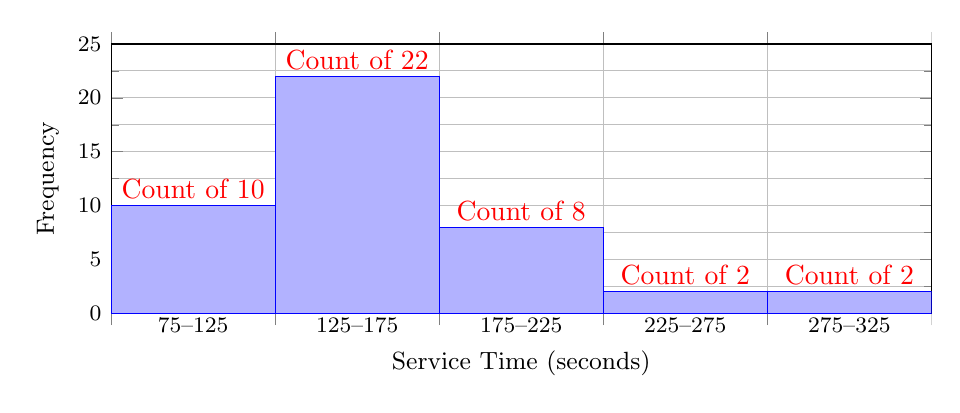
\begin{tikzpicture}
\begin{axis}[
small,
height=5.0cm,
width=12.0cm,
enlarge x limits=false,
enlarge y limits=false,
ybar interval,
ymajorgrids=true,
minor y tick num=1,
yminorgrids=true,
ylabel={Frequency},
xlabel={Service Time (seconds)},
x tick label style={rotate=0,anchor=center},
xtick={75, 125,...,325},
ytick={0,5,...,1000},
ymin=0,
ymax=25,
xmin=75,
xmax=325,
xticklabel style={/pgf/number format/.cd,fixed,precision=0},
xticklabel=
\pgfmathprintnumber\tick--\pgfmathprintnumber\nexttick,
]
\only<beamer:7|handout:1>{%
\draw [blue,fill=blue!30!white] (axis cs: 75,0) rectangle (axis cs: 125,10);
\draw [blue,fill=blue!30!white] (axis cs: 125,0) rectangle (axis cs: 175,22);
\draw [blue,fill=blue!30!white] (axis cs: 175,0) rectangle (axis cs: 225,8);
\draw [blue,fill=blue!30!white] (axis cs: 225,0) rectangle (axis cs: 275,2);
\draw [blue,fill=blue!30!white] (axis cs: 275,0) rectangle (axis cs: 325,2);
}
\temporal<2| handout:0>{\draw [style={opacity=0}] (axis cs: 75,0) rectangle (axis cs: 125,10);}%
                     {\draw [blue,fill=red] (axis cs: 75,0) rectangle (axis cs: 125,10);
                      \path (axis cs: 75,10) --  (axis cs: 125,10) node[red,midway,above,yshift = -1pt] {Count of 10};}%
                     {\draw [blue,fill=blue!30!white] (axis cs: 75,0) rectangle (axis cs: 125,10);}%
\temporal<3| handout:0>{\draw [style={opacity=0}] (axis cs: 125,0) rectangle (axis cs: 175,22);}%
                     {\draw [blue,fill=red] (axis cs: 125,0) rectangle (axis cs: 175,22);
                      \path (axis cs: 125,22) --  (axis cs: 175,22) node[red,midway,above,yshift = -1pt] {Count of 22};}%
                     {\draw [blue,fill=blue!30!white] (axis cs: 125,0) rectangle (axis cs: 175,22);}%
\temporal<4| handout:0>{\draw [style={opacity=0}] (axis cs: 175,0) rectangle (axis cs: 225,8);}%
                     {\draw [blue,fill=red] (axis cs: 175,0) rectangle (axis cs: 225,8);
                      \path (axis cs: 175,8) --  (axis cs: 225,8) node[red,midway,above,yshift = -1pt] {Count of 8};}%
                     {\draw [blue,fill=blue!30!white] (axis cs: 175,0) rectangle (axis cs: 225,8);}%
\temporal<5| handout:0>{\draw [style={opacity=0}] (axis cs: 225,0) rectangle (axis cs: 275,2);}%
                     {\draw [blue,fill=red] (axis cs: 225,0) rectangle (axis cs: 275,2);
                      \path (axis cs: 225,2) --  (axis cs: 275,2) node[red,midway,above,yshift = -1pt] {Count of 2};}%
                     {\draw [blue,fill=blue!30!white] (axis cs: 225,0) rectangle (axis cs: 275,2);}%
\temporal<6| handout:0>{\draw [style={opacity=0}] (axis cs: 275,0) rectangle (axis cs: 325,2);}%
                     {\draw [blue,fill=red] (axis cs: 275,0) rectangle (axis cs: 325,2);
                      \path (axis cs: 275,2) --  (axis cs: 325,2) node[red,midway,above,yshift = -1pt] {Count of 2};}%
                     {\draw [blue,fill=blue!30!white] (axis cs: 275,0) rectangle (axis cs: 325,2);}%
\end{axis}
\end{tikzpicture}
\end{center}
\end{example}
\onslide<7>
\end{frame}

\begin{frame}
\begin{example}
\begin{center}
\begin{tikzpicture}
\begin{axis}[
small,
height=4.5cm,
width=12.0cm,
enlarge x limits=true,
enlarge y limits=false,
%ybar interval,
grid=both,
minor y tick num=1,
minor x tick num=1,
ylabel={Frequency},
xlabel={Interest Rate},
%x tick label style={rotate=0,anchor=south east},
tick align=outside, % <-- this positions the ticks "outside"
xtick={5, 10,...,30},
ytick={0,5,...,15},
ymin=0,
ymax=15,
xmin=5,
xmax=30,
xticklabel style={/pgf/number format/.cd,fixed,precision=0},
xticklabel=
\pgfmathprintnumber\tick\%,%--\pgfmathprintnumber\nexttick\%,
]
%\draw[red] (axis cs: 5,-1) -- (axis cs: 5,16);
%\draw[red] (axis cs: 10,0) -- (axis cs: 10,15);
%\draw[red] (axis cs: 15,0) -- (axis cs: 15,15);
%\draw[red] (axis cs: 20,0) -- (axis cs: 20,15);
%\draw[red] (axis cs: 25,0) -- (axis cs: 25,15);
\addplot+ [ybar interval, mark=none, fill=blue!30!white, hist={bins=10, data min=5, data max=30}]
table [y=interest_rate, col sep=comma] {loan50.csv};
\end{axis}
\end{tikzpicture}
\end{center}

\begin{center}
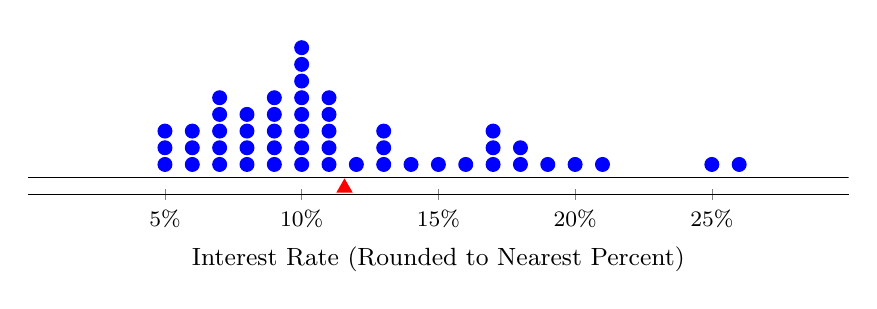
\begin{tikzpicture}
\pgfplotsset{ every non boxed x axis/.append style={x axis line style=-},
     every non boxed y axis/.append style={y axis line style=-}}
\begin{axis}[
small,
width=12cm,
height=3.7cm,
xlabel={Interest Rate (Rounded to Nearest Percent)},
ylabel={},
yticklabels={},
axis y line=none,
axis x line=bottom,
xticklabel=\pgfmathprintnumber{\tick}\%,
xtick={5,10,15,20,25},
ymin=0,
ymax=10,
xmin=0,
xmax=30,
scatter/use mapped color={
 %draw=mapped color,
 fill=blue,
},
]
\addplot [domain=0:30]  {1};
\addplot[scatter, only marks, blue, scatter src=y, mark size=2.5pt]
coordinates
{
(11, 1.8)
(11, 2.8)
(11, 3.8)
(11, 4.8)
(11, 5.8)
(10, 1.8)
(10, 2.8)
(10, 3.8)
(10, 4.8)
(10, 5.8)
(10, 6.8)
(10, 7.8)
(10, 8.8)
(26, 1.8)
(9, 1.8)
(9, 2.8)
(9, 3.8)
(9, 4.8)
(9, 5.8)
(17, 1.8)
(17, 2.8)
(17, 3.8)
(6, 1.8)
(6, 2.8)
(6, 3.8)
(8, 1.8)
(8, 2.8)
(8, 3.8)
(8, 4.8)
(13, 1.8)
(13, 2.8)
(13, 3.8)
(5, 1.8)
(5, 2.8)
(5, 3.8)
(7, 1.8)
(7, 2.8)
(7, 3.8)
(7, 4.8)
(7, 5.8)
(25, 1.8)
(18, 1.8)
(18, 2.8)
(19, 1.8)
(14, 1.8)
(20, 1.8)
(15, 1.8)
(12, 1.8)
(16, 1.8)
(21, 1.8)
};
\addplot [scatter, only marks, red, scatter src=y, mark size=3pt, scatter/use mapped color={fill=red,}, mark=triangle*] coordinates {(11.567, 0.4)};
\end{axis}
\end{tikzpicture}
\end{center}
\end{example}
\end{frame}

\begin{frame}
\begin{definition}
If all of the bars in a histogram are close to the same height, then the distribution is said to be \textbf{uniformly distributed}.
\end{definition}

\begin{example}
\begin{center}
\begin{tikzpicture}
\begin{axis}[
small,
height=7.0cm,
width=11.75cm,
enlarge x limits=false,
enlarge y limits=false,
ybar interval,
ymajorgrids=true,
minor y tick num=1,
yminorgrids=true,
ylabel={Frequency},
xlabel={},
x tick label style={rotate=0,anchor=center},
%xtick={0,1,2,3,4,5,6,7,8,9},
%ytick={0,1,...,10},
ymin=0,
ymax=1100,
%xmin=0,
%xmax=9,
%xticklabel style={/pgf/number format/.cd,fixed,precision=0},
%xticklabel=
%\pgfmathprintnumber\tick--\pgfmathprintnumber\nexttick,
%yticklabel style={/pgf/number format/.cd,fixed,precision=0},
%yticklabel=
%\pgfmathprintnumber\tick\%
]
\addplot+ [hist={bins=10, data min=0, data max=10}]
table [y=nums] {randu.dat};
\end{axis}
\end{tikzpicture}
\end{center}
\end{example}
\end{frame}

\begin{frame}
\begin{definition}
When the data trails off to the right and has a longer right tail, the distribution is said to be \textbf{right skewed}.
\end{definition}
\begin{example}
\begin{center}
\begin{tikzpicture}
\begin{axis}[
small,
height=7.0cm,
width=12cm,
enlarge x limits=false,
enlarge y limits=false,
ybar interval,
ymajorgrids=true,
minor y tick num=1,
yminorgrids=true,
ylabel={Frequency},
xlabel={},
x tick label style={rotate=0,anchor=center},
xtick={0,10,...,60},
%ytick={0,1,...,10},
ymin=0,
ymax=700,
%xmin=0,
%xmax=9,
%xticklabel style={/pgf/number format/.cd,fixed,precision=0},
%xticklabel=
%\pgfmathprintnumber\tick--\pgfmathprintnumber\nexttick,
%yticklabel style={/pgf/number format/.cd,fixed,precision=0},
%yticklabel=
%\pgfmathprintnumber\tick\%
]
\addplot+ [hist={bins=60, data min=0, data max=60}]
table [y=nums] {randsr.dat};
\end{axis}
\end{tikzpicture}
\end{center}
\end{example}
\end{frame}

\begin{frame}
\begin{definition}
When the data trails off to the left and has a longer left tail, the distribution is said to be \textbf{left skewed}.
\end{definition}
\begin{example}
\begin{center}
\begin{tikzpicture}
\begin{axis}[
small,
height=7.0cm,
width=12cm,
enlarge x limits=false,
enlarge y limits=false,
ybar interval,
ymajorgrids=true,
minor y tick num=1,
yminorgrids=true,
ylabel={Frequency},
xlabel={},
x tick label style={rotate=0,anchor=center},
xtick={0,10,...,60},
%ytick={0,1,...,10},
ymin=0,
ymax=700,
%xmin=0,
%xmax=9,
%xticklabel style={/pgf/number format/.cd,fixed,precision=0},
%xticklabel=
%\pgfmathprintnumber\tick--\pgfmathprintnumber\nexttick,
%yticklabel style={/pgf/number format/.cd,fixed,precision=0},
%yticklabel=
%\pgfmathprintnumber\tick\%
]
\addplot+ [hist={bins=60, data min=0, data max=60}]
table [y=nums] {randsl.dat};
\end{axis}
\end{tikzpicture}
\end{center}
\end{example}
\end{frame}

\begin{frame}
\begin{note}
\begin{columns}
\begin{column}{0.18\textwidth}
Skewed to the left resembles the toes on your left foot.
\end{column}
\begin{column}{0.54\textwidth}
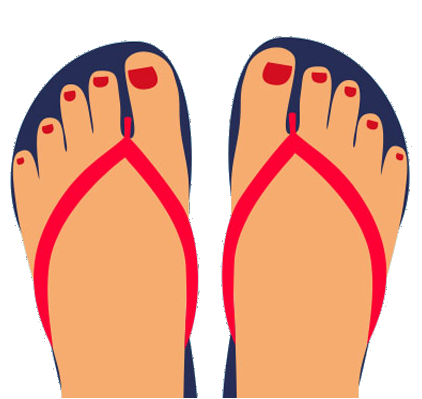
\includegraphics[width=\textwidth]{feet.png}
\end{column}
\begin{column}{0.18\textwidth}
Skewed to the right resembles the toes on your right foot.
\end{column}
\end{columns}
\end{note}\pause

\begin{definition}
If the distribution of data is skewed to the left or skewed to the right, the distribution is called \textbf{skewed}.
\end{definition}
\end{frame}

\begin{frame}
\begin{definition}
Data sets that show roughly equal trailing off in both directions are called \textbf{symmetric}.
\end{definition}
\begin{example}
\begin{center}
\begin{tikzpicture}
\begin{axis}[
small,
height=6.7cm,
width=12.0cm,
enlarge x limits=false,
enlarge y limits=false,
ybar interval,
ymajorgrids=true,
minor y tick num=1,
yminorgrids=true,
ylabel={Frequency},
xlabel={},
%x tick label style={rotate=0,anchor=center},
xtick={10,20,...,500},
%ytick={0,10,...,1000},
xmin=0,
xmax=190,
ymin=0,
ymax=500
%xticklabel style={/pgf/number format/.cd,fixed,precision=0},
%xticklabel=
%\pgfmathprintnumber\tick--\pgfmathprintnumber\nexttick,
%yticklabel style={/pgf/number format/.cd,fixed,precision=0},
%yticklabel=
%\pgfmathprintnumber\tick\%
]
\addplot+ [hist={bins=75}]
table [y=nums] {randn.dat};
\end{axis}
\end{tikzpicture}
\end{center}
\end{example}
\end{frame}

\begin{frame}
\begin{definition}
A \textbf{mode} is represented by a prominent peak in the distribution.
\end{definition}\pause

\begin{definition}
If a distribution has exactly one mode, it is called \textbf{unimodal}.
\end{definition}\pause

\begin{definition}
If the distribution has exactly two modes, it is called \textbf{bimodal}.
\end{definition}\pause

\begin{definition}
If the distribution has more than two modes, it is called \textbf{multimodal}.
\end{definition}
\end{frame}

\begin{frame}
\begin{example}
\begin{center}
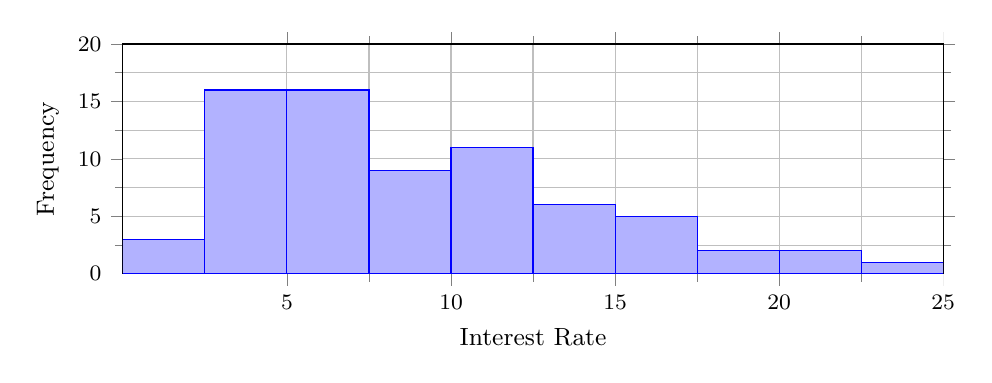
\begin{tikzpicture}
\begin{axis}[
small,
height=4.5cm,
width=12.0cm,
enlarge x limits=false,
enlarge y limits=false,
%ybar interval,
grid=both,
minor y tick num=1,
minor x tick num=1,
ylabel={Frequency},
xlabel={Interest Rate},
%x tick label style={rotate=0,anchor=south east},
tick align=outside, % <-- this positions the ticks "outside"
xtick={5, 10,...,30},
ytick={0,5,...,20},
ymin=0,
ymax=20,
xmin=0,
xmax=25,
xticklabel style={/pgf/number format/.cd,fixed,precision=0},
xticklabel=
\pgfmathprintnumber\tick,%--\pgfmathprintnumber\nexttick\%,
]
\draw [blue,fill=blue!30!white] (axis cs: 0,0) rectangle (axis cs: 2.5,3);
\draw [blue,fill=blue!30!white] (axis cs: 2.5,0) rectangle (axis cs: 5,16);
\draw [blue,fill=blue!30!white] (axis cs: 5,0) rectangle (axis cs: 7.5,16);
\draw [blue,fill=blue!30!white] (axis cs: 7.5,0) rectangle (axis cs: 10,9);
\draw [blue,fill=blue!30!white] (axis cs: 10,0) rectangle (axis cs: 12.5,11);
\draw [blue,fill=blue!30!white] (axis cs: 12.5,0) rectangle (axis cs: 15,6);
\draw [blue,fill=blue!30!white] (axis cs: 15,0) rectangle (axis cs: 17.5,5);
\draw [blue,fill=blue!30!white] (axis cs: 17.5,0) rectangle (axis cs: 20,2);
\draw [blue,fill=blue!30!white] (axis cs: 20,0) rectangle (axis cs: 22.5,2);
\draw [blue,fill=blue!30!white] (axis cs: 22.5,0) rectangle (axis cs: 25,1);
\end{axis}
\end{tikzpicture}
\end{center}
\question{How many modes does this distribution have?}\pause
\answer{One}\pause

\vspace{1mm}
\question{Is this distribution unimodal, bimodal, or multimodal?}\pause
\answer{Unimodal}
\end{example}
\end{frame}

\begin{frame}
\begin{example}
\begin{center}
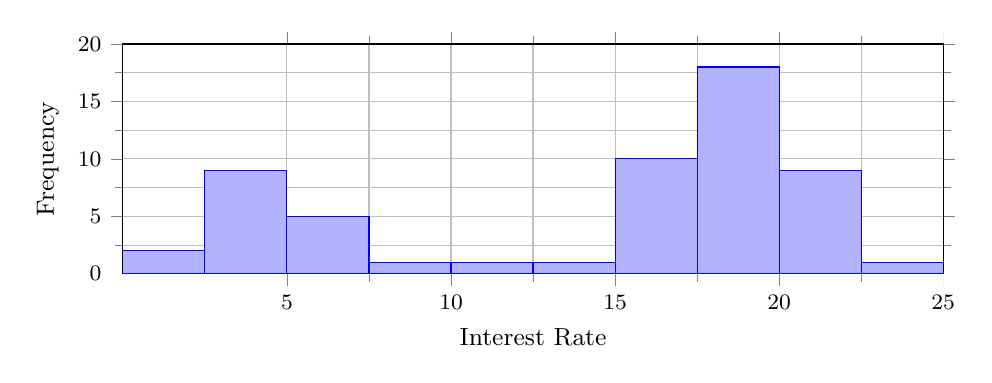
\begin{tikzpicture}
\begin{axis}[
small,
height=4.5cm,
width=12.0cm,
enlarge x limits=false,
enlarge y limits=false,
%ybar interval,
grid=both,
minor y tick num=1,
minor x tick num=1,
ylabel={Frequency},
xlabel={Interest Rate},
%x tick label style={rotate=0,anchor=south east},
tick align=outside, % <-- this positions the ticks "outside"
xtick={5, 10,...,30},
ytick={0,5,...,20},
ymin=0,
ymax=20,
xmin=0,
xmax=25,
xticklabel style={/pgf/number format/.cd,fixed,precision=0},
xticklabel=
\pgfmathprintnumber\tick,%--\pgfmathprintnumber\nexttick\%,
]
\draw [blue,fill=blue!30!white] (axis cs: 0,0) rectangle (axis cs: 2.5,2);
\draw [blue,fill=blue!30!white] (axis cs: 2.5,0) rectangle (axis cs: 5,9);
\draw [blue,fill=blue!30!white] (axis cs: 5,0) rectangle (axis cs: 7.5,5);
\draw [blue,fill=blue!30!white] (axis cs: 7.5,0) rectangle (axis cs: 10,1);
\draw [blue,fill=blue!30!white] (axis cs: 10,0) rectangle (axis cs: 12.5,1);
\draw [blue,fill=blue!30!white] (axis cs: 12.5,0) rectangle (axis cs: 15,1);
\draw [blue,fill=blue!30!white] (axis cs: 15,0) rectangle (axis cs: 17.5,10);
\draw [blue,fill=blue!30!white] (axis cs: 17.5,0) rectangle (axis cs: 20,18);
\draw [blue,fill=blue!30!white] (axis cs: 20,0) rectangle (axis cs: 22.5,9);
\draw [blue,fill=blue!30!white] (axis cs: 22.5,0) rectangle (axis cs: 25,1);
\end{axis}
\end{tikzpicture}
\end{center}
\question{How many modes does this distribution have?}\pause
\answer{Two}\pause

\vspace{1mm}
\question{Is this distribution unimodal, bimodal, or multimodal?}\pause
\answer{Bimodal}
\end{example}
\end{frame}

\begin{frame}
\begin{example}
\begin{center}
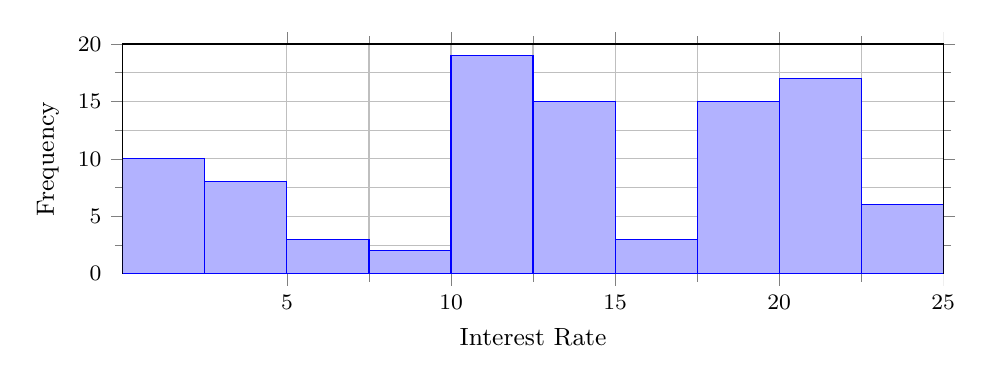
\begin{tikzpicture}
\begin{axis}[
small,
height=4.5cm,
width=12.0cm,
enlarge x limits=false,
enlarge y limits=false,
%ybar interval,
grid=both,
minor y tick num=1,
minor x tick num=1,
ylabel={Frequency},
xlabel={Interest Rate},
%x tick label style={rotate=0,anchor=south east},
tick align=outside, % <-- this positions the ticks "outside"
xtick={5, 10,...,30},
ytick={0,5,...,20},
ymin=0,
ymax=20,
xmin=0,
xmax=25,
xticklabel style={/pgf/number format/.cd,fixed,precision=0},
xticklabel=
\pgfmathprintnumber\tick,%--\pgfmathprintnumber\nexttick\%,
]
\draw [blue,fill=blue!30!white] (axis cs: 0,0) rectangle (axis cs: 2.5,10);
\draw [blue,fill=blue!30!white] (axis cs: 2.5,0) rectangle (axis cs: 5,8);
\draw [blue,fill=blue!30!white] (axis cs: 5,0) rectangle (axis cs: 7.5,3);
\draw [blue,fill=blue!30!white] (axis cs: 7.5,0) rectangle (axis cs: 10,2);
\draw [blue,fill=blue!30!white] (axis cs: 10,0) rectangle (axis cs: 12.5,19);
\draw [blue,fill=blue!30!white] (axis cs: 12.5,0) rectangle (axis cs: 15,15);
\draw [blue,fill=blue!30!white] (axis cs: 15,0) rectangle (axis cs: 17.5,3);
\draw [blue,fill=blue!30!white] (axis cs: 17.5,0) rectangle (axis cs: 20,15);
\draw [blue,fill=blue!30!white] (axis cs: 20,0) rectangle (axis cs: 22.5,17);
\draw [blue,fill=blue!30!white] (axis cs: 22.5,0) rectangle (axis cs: 25,6);
\end{axis}
\end{tikzpicture}
\end{center}
\question{How many modes does this distribution have?}\pause
\answer{Three}\pause

\vspace{1mm}
\question{Is this distribution unimodal, bimodal, or multimodal?}\pause
\answer{Multimodal}
\end{example}
\end{frame}

\begin{frame}
\begin{example}
Let us consider the weights of randomly selected pennies.
\begin{center}
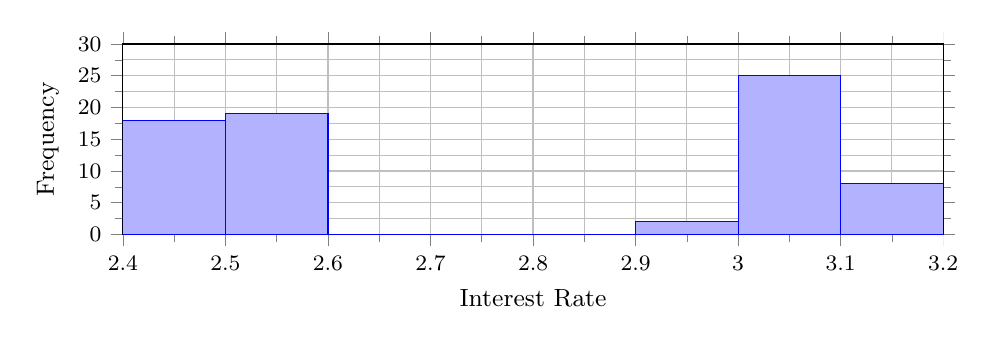
\begin{tikzpicture}
\begin{axis}[
small,
height=4cm,
width=12.0cm,
enlarge x limits=false,
enlarge y limits=false,
%ybar interval,
grid=both,
minor y tick num=1,
minor x tick num=1,
ylabel={Frequency},
xlabel={Interest Rate},
%x tick label style={rotate=0,anchor=south east},
tick align=outside, % <-- this positions the ticks "outside"
xtick={2.4,2.5,...,3.3},
ytick={0,5,...,30},
ymin=0,
ymax=30,
xmin=2.4,
xmax=3.2,
xticklabel style={/pgf/number format/.cd,fixed,precision=1},
xticklabel=
\pgfmathprintnumber\tick,%--\pgfmathprintnumber\nexttick\%,
]
\draw [blue,fill=blue!30!white] (axis cs: 2.4,0) rectangle (axis cs: 2.5,18);
\draw [blue,fill=blue!30!white] (axis cs: 2.5,0) rectangle (axis cs: 2.6,19);
\draw [blue,fill=blue!30!white] (axis cs: 2.6,0) rectangle (axis cs: 2.7,0);
\draw [blue,fill=blue!30!white] (axis cs: 2.7,0) rectangle (axis cs: 2.8,0);
\draw [blue,fill=blue!30!white] (axis cs: 2.8,0) rectangle (axis cs: 2.9,0);
\draw [blue,fill=blue!30!white] (axis cs: 2.9,0) rectangle (axis cs: 3.0,2);
\draw [blue,fill=blue!30!white] (axis cs: 3.0,0) rectangle (axis cs: 3.1,25);
\draw [blue,fill=blue!30!white] (axis cs: 3.1,0) rectangle (axis cs: 3.2,8);
\end{axis}
\end{tikzpicture}
\end{center}
\question{How many modes does this distribution have?}\pause
\answer{Two}\pause

\vspace{1mm}
The modes describe two different types of pennies in circulation:
\begin{itemize}
\item Pennies made before 1983 are 95\% copper and 5\% zinc.
\item Pennies made after 1983 are 2.5\% copper and 97.5\% zinc.
\end{itemize}
Since copper is more dense than zinc, pennies made after 1983 weigh less.
\end{example}
\end{frame}

\begin{frame}[fragile]
\begin{example}
Consider the waiting times at a bank.

\vspace{-3mm}
\begin{center}
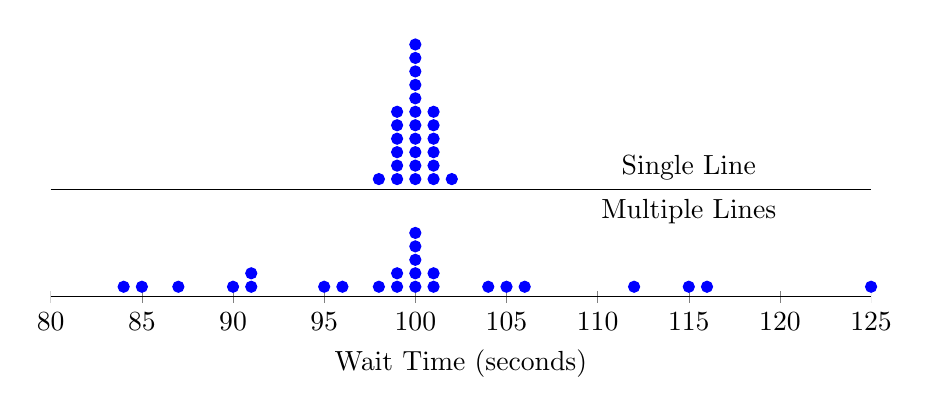
\begin{tikzpicture}
\pgfplotsset{ every non boxed x axis/.append style={x axis line style=-},
     every non boxed y axis/.append style={y axis line style=-}}
\begin{axis}[
width=12cm,
height=5cm,
xlabel={Wait Time (seconds)},
ylabel={},
yticklabels={},
axis y line=none,
axis x line=bottom,
ymin=0,
ymax=20,
xmin=80,
xmax=125,
scatter/use mapped color={
 %draw=mapped color,
 fill=blue,
},
]
\addplot[scatter, only marks, blue, scatter src=y]
coordinates
{
(84, 0.75)
(85, 0.75)
(87, 0.75)
(90, 0.75)
(91, 0.75)
(91, 1.75)
(95, 0.75)
(96, 0.75)
(98, 0.75)
(99, 0.75)
(99, 1.75)
(100, 0.75)
(100, 1.75)
(100, 2.75)
(100, 3.75)
(100, 4.75)
(101, 0.75)
(101, 1.75)
(104, 0.75)
(105, 0.75)
(106, 0.75)
(112, 0.75)
(115, 0.75)
(116, 0.75)
(125, 0.75)
};

\draw (axis cs:80,8) -- (axis cs:125,8);
\draw (axis cs:115,8) node[above]{Single Line};
\draw (axis cs:115,8) node[below]{Multiple Lines};

\addplot[scatter, only marks, blue, scatter src=y]
coordinates
{
(98, 8.75)
(99, 8.75)
(99, 9.75)
(99, 10.75)
(99, 11.75)
(99, 12.75)
(99, 13.75)
(100, 8.75)
(100, 9.75)
(100, 10.75)
(100, 11.75)
(100, 12.75)
(100, 13.75)
(100, 14.75)
(100, 15.75)
(100, 16.75)
(100, 17.75)
(100, 18.75)
(101, 8.75)
(101, 9.75)
(101, 10.75)
(101, 11.75)
(101, 12.75)
(101, 13.75)
(102, 8.75)
};
\end{axis}
\end{tikzpicture}
\end{center}\pause

\vspace{-3mm}
Both of these data sets have the same mean, but they are very different.
\end{example}\pause

\begin{definition}
A \textbf{measure of variation} describes how spread out a distribution is.
\end{definition}
\end{frame}

\begin{frame}
\begin{definition}
The distance between an observation and it's mean is called it's \textbf{deviation}. You calculate the deviation as: $x-\bar{x}$.
\end{definition}\pause

\begin{example}
Recall that the mean of \texttt{interest\_rate} is $11.57$\%.
\begin{center}
\begin{tabular}{ll}
data & deviation \\\hline\pause
10.90 & $x_1-\bar{x} = 10.90 - 11.57 = -0.67$ \\\pause
9.92 & $x_2-\bar{x}=9.92-11.57=-1.65$ \\\pause
26.30 & $x_3-\bar{x}=26.30-11.57=14.73$ \\\pause
&\vdots\\
6.08 & $x_{50}-\bar{x}=6.08-11.57=-5.49$\pause
\end{tabular}
\end{center}
\end{example}

\begin{note}
A positive deviation means the data value is larger than the mean.\\ A negative deviation means the data value is smaller than the mean.
\end{note}
\end{frame}

\begin{frame}
\begin{definition}
The \textbf{variance} of a sample, denoted as $s^2$, is
\begin{equation*}
s^2 = \dfrac{\sum \left(x-\bar{x}\right)}{n-1}
\end{equation*}
\end{definition}\pause

\begin{note}
When computing a variance of a population, you divide by $N$ instead of $n-1$ for fiddly mathematical reasons.
\end{note}\pause

\begin{definition}
The \textbf{standard deviation}, denoted $s$, is the square root of the variance.
\end{definition}\pause

\begin{note}
The standard deviation of a population is denoted $\sigma$ and variance $\sigma^2$.
\end{note}
\end{frame}

\begin{frame}
\begin{example}
The variance of \texttt{interest\_rate} is
\begin{equation*}
\begin{aligned}
s^2 &= \dfrac{\sum \left(x-\bar{x}\right)}{n-1}\\\pause
&=  \dfrac{{(-0.67)}^2+{(-1.65)}^2+{(14.73)}^2+\cdots+{(-5.49)}^2}{50-1}  \\\pause
&= \dfrac{0.45+2.72+216.97+\cdots+30.14}{49} \\\pause
&= 25.524\pause
\end{aligned}
\end{equation*}
The standard deviation of \texttt{interest\_rate} is
\begin{equation*}
\begin{aligned}
s &= \sqrt{s^2} \pause = \sqrt{25.524} \pause = 5.052
\end{aligned}
\end{equation*}
\end{example}\pause
\begin{note}
Computers are often used to compute variance and standard deviation.
\end{note}
\end{frame}

\begin{frame}
\begin{block}{Properties}
\begin{itemize}[<+- | alert@+>]
\item The standard deviation is a measure of how much most of the data values deviate from the mean.
\item The value of the standard deviation is never negative.
\item The value of the standard deviation is only zero when all of the data values are exactly the same.
\item Larger values of s indicate greater amounts of variation.
\item The standard deviation can increase dramatically with one or more extreme values.
\item The units of the standard deviation are the same units as the original data values.
\end{itemize}
\end{block}
\onslide<+->
\begin{note}
For reason will explore in Chapter 4, we expect most of the data to fall within one standard deviation of the mean.
\end{note}
\end{frame}

\begin{frame}
\begin{definition}
\textbf{Percentiles} are measures of location, denoted $P_{1},P_{2},\ldots,P_{99}$, which divide a set of data into 100 groups with about $1\%$ of the values in each group.
\end{definition}\pause

\begin{block}{Formula}
The process of finding the percentile that corresponds to a particular data value $x$ is given by the following:
\begin{equation*}
\text{Percentile of value $x$} = \dfrac{\text{number of values less than $x$}}{\text{total number of values}}\cdot 100
\end{equation*}
\end{block}\pause

\begin{note}
Round percentiles to the nearest whole number.
\end{note}
\end{frame}

\begin{frame}
\begin{example}
The table lists the 50 smartphone data speeds, in Mbps.
\begin{center}
\begin{tabular}{rrrrrrrrrr}
38.5 & 55.6 & 22.4 & 14.1 & 23.1 & 24.5 & \textcolor<2->{blue}{6.5} & 21.5 & 25.7 & 14.7 \\
77.8 & 71.3 & 43.0 & 20.2 & 15.5 & 13.7 & \textcolor<2->{blue}{11.1} & 13.5 & \textcolor<2->{blue}{10.2} & 21.1 \\
15.1 & 14.2 & \textcolor<2->{blue}{4.5} & \textcolor<2->{blue}{7.9} & \textcolor<2->{blue}{9.9} & \textcolor<2->{blue}{10.3} & \textcolor<2->{blue}{6.2} & 17.5 & 22.2 & 13.1 \\
18.2 & 28.5 & 15.8 & 15.0 & \textcolor<2->{blue}{11.1} & \textcolor<2->{red}{11.8} & 16.0 & \textcolor<2->{blue}{10.9} & \textcolor<2->{blue}{1.8} & 34.6 \\
\textcolor<2->{blue}{4.6} & 12.0 & \textcolor<2->{blue}{11.6} & \textcolor<2->{blue}{3.6} & \textcolor<2->{blue}{1.9} & \textcolor<2->{blue}{7.7} & \textcolor<2->{blue}{0.8} & \textcolor<2->{blue}{4.5} & \textcolor<2->{blue}{1.4} & \textcolor<2->{blue}{3.2} \\
\end{tabular}
\end{center}
Let us find which percentile the data value 11.8 Mbps in.\pause

\vspace{1mm}
There are 20 \textcolor{blue}{data values less than} \textcolor{red}{11.8} Mbps.\pause 

\vspace{-3mm}
\begin{equation*}
\text{Percentile of}~\textcolor{red}{11.8}=\dfrac{20}{50}\cdot 100 = 40\pause
\end{equation*}

\vspace{-5mm}
A data speed of 11.8 Mbps is in the 40th percentile.
\end{example}\pause

\begin{note}
This can be interpreted loosely as 40\% of the data speeds are slower than 11.8 Mbps and 60\% of the data speeds are faster than 11.8 Mbps.
\end{note}
\end{frame}

\begin{frame}
\begin{block}{Converting a Percentile to a Data Value}
Notation:
\begin{itemize}
\item $n$ is the total number of values in the data set.
\item $k$ is the percentile being used.
\item $L$ is the locator that gives the position of a value.
\item $P_k$ is the $k$th percentile.
\end{itemize}\pause
To find which data value is in the $P_k$ percentile:
\begin{enumerate}
\item Sort the data from lowest to highest.\pause
\item Compute $L=\left(\dfrac{k}{100}\right)n$\pause
\item \begin{itemize}
\item If $L$ is a whole number, the value of the $k$th percentile is midway between the $L$th value and the next value in the sorted data. Add the $L$th value and $(L+1)$th value, then divide by 2.\pause
\item If $L$ is not a whole number, round $L$ up to the nearest whole number. $P_k$is the $L$th data value. 
\end{itemize}
\end{enumerate}
\end{block}
\end{frame}

\begin{frame}
\begin{example}
The table lists the \textcolor<4-5|handout:0>{red}{50} Verizon airport data speeds, in Mbps, from\\ Data Set 32 in Appendix B.
\temporal<2-6>{%
\begin{center}
\begin{tabular}{|rrrrrrrrrr|}\hline
38.5 & 55.6 & 22.4 & 14.1 & 23.1 & 24.5 & 6.5 & 21.5 & 25.7 & 14.7 \\
77.8 & 71.3 & 43.0 & 20.2 & 15.5 & 13.7 & 11.1 & 13.5 & 10.2 & 21.1 \\
15.1 & 14.2 & 4.5 & 7.9 & 9.9 & 10.3 & 6.2 & 17.5 & 22.2 & 13.1 \\
18.2 & 28.5 & 15.8 & 15.0 & 11.1 & 11.8 & 16.0 & 10.9 & 1.8 & 34.6 \\
4.6 & 12.0 & 11.6 & 3.6 & 1.9 & 7.7 & 0.8 & 4.5 & 1.4 & 3.2 \\\hline
\end{tabular}
\end{center}
}{%
\begin{center}
\begin{tabular}{|rrrrrrrrrr|}\hline
0.8 & 1.4 & 1.8 & 1.9 & 3.2 & 3.6 & 4.5 & 4.5 & 4.6 & 6.2 \\
6.5 & 7.7 & 7.9 & 9.9 & 10.2 & 10.3 & 10.9 & 11.1 & 11.1 & 11.6 \\
11.8 & 12.0 & 13.1 & 13.5 & 13.7 & 14.1 & 14.2 & 14.7 & 15.0 & 15.1 \\
15.5 & 15.8 & 16.0 & 17.5 & 18.2 & 20.2 & 21.1 & 21.5 & 22.2 & 22.4 \\
23.1 & 24.5 & 25.7 & 28.5 & 34.6 & 38.5 & 43.0 & 55.6 & 71.3 & 77.8 \\\hline
\end{tabular}
\end{center}
}{%
\begin{center}
\begin{tabular}{|rrrrrrrrrr|}\hline
\textcolor<2->{blue}{0.8} &
\textcolor<2->{blue}{1.4} &
\textcolor<2->{blue}{1.8} &
\textcolor<2->{blue}{1.9} &
\textcolor<2->{blue}{3.2} &
\textcolor<2->{blue}{3.6} &
\textcolor<2->{blue}{4.5} &
\textcolor<2->{blue}{4.5} &
\textcolor<2->{blue}{4.6} &
\textcolor<2->{blue}{6.2} \\
\textcolor<2->{blue}{6.5} &
\textcolor<2->{blue}{7.7} &
\textcolor<2->{red}{7.9} &
\textcolor<2->{cyan}{9.9} &
\textcolor<2->{cyan}{10.2} &
\textcolor<2->{cyan}{10.3} &
\textcolor<2->{cyan}{10.9} &
\textcolor<2->{cyan}{11.1} &
\textcolor<2->{cyan}{11.1} &
\textcolor<2->{cyan}{11.6} \\
\textcolor<2->{cyan}{11.8} &
\textcolor<2->{cyan}{12.0} &
\textcolor<2->{cyan}{13.1} &
\textcolor<2->{cyan}{13.5} &
\textcolor<2->{cyan}{13.7} &
\textcolor<2->{cyan}{14.1} &
\textcolor<2->{cyan}{14.2} &
\textcolor<2->{cyan}{14.7} &
\textcolor<2->{cyan}{15.0} &
\textcolor<2->{cyan}{15.1} \\
\textcolor<2->{cyan}{15.5} &
\textcolor<2->{cyan}{15.8} &
\textcolor<2->{cyan}{16.0} &
\textcolor<2->{cyan}{17.5} &
\textcolor<2->{cyan}{18.2} &
\textcolor<2->{cyan}{20.2} &
\textcolor<2->{cyan}{21.1} &
\textcolor<2->{cyan}{21.5} &
\textcolor<2->{cyan}{22.2} &
\textcolor<2->{cyan}{22.4} \\
\textcolor<2->{cyan}{23.1} &
\textcolor<2->{cyan}{24.5} &
\textcolor<2->{cyan}{25.7} &
\textcolor<2->{cyan}{28.5} &
\textcolor<2->{cyan}{34.6} &
\textcolor<2->{cyan}{38.5} &
\textcolor<2->{cyan}{43.0} &
\textcolor<2->{cyan}{55.6} &
\textcolor<2->{cyan}{71.3} &
\textcolor<2->{cyan}{77.8} \\\hline
\end{tabular}
\end{center}
}
Let us find which value is in the \textcolor<4-5|handout:0>{blue}{25}th percentile, $P_{25}$.\pause

\vspace{1mm}
First, sort the data.\pause

\vspace{1mm}
We next need to compute
\begin{equation*}
L=\dfrac{k}{100}\cdot n\pause
=\dfrac{\textcolor<4-5|handout:0>{blue}{25}}{100}\cdot \textcolor<4-5|handout:0>{red}{50}\pause
=12.5\pause
\end{equation*}
Since $L=12.5$ is not a whole number, we round up to $13$.\pause

\vspace{1mm}
So, $P_{25}$ is the 13th data value, \textcolor<7-|handout:0>{red}{7.9} Mbps.
\end{example}
\end{frame}

\begin{frame}
\begin{definition}
\textbf{Quartiles} are measures of location, denoted $Q_1$, $Q_2$, and $Q_3$, which divide a set of data into four groups with about 25\% of the values in each group.
\end{definition}\pause

\begin{block}{Quartile Descriptions}
\begin{description}
\item[\textbf{First Quartile, $\boldsymbol{Q_1}$:}] Same value as $P_{25}$. It separates the bottom 25\% of the sorted values from the top 75\%.\pause
\item[\textbf{Second Quartile, $\boldsymbol{Q_2}$:}] Same as the $P_{50}$ and the median. It separates the bottom 50\% of the sorted values from the top 50\%\pause
\item[\textbf{Third Quartile, $\boldsymbol{Q_3}$}:] Same as $P_{75}$. It separates the bottom 75\% of the sorted values from the top 25\%.
\end{description}
\end{block}\pause

\begin{note}
Use the same procedure for calculating percentiles to calculate quartiles.
\end{note}
\end{frame}


\begin{frame}
\begin{definition}
For a set of data, the \textbf{5-number summary} consists of the five values:
\begin{enumerate}
\item Minimum
\item $Q_1$
\item Median ($Q_2$)
\item $Q_3$
\item Maximum
\end{enumerate}
\end{definition}\pause

\begin{definition}
A \textbf{boxplot} is a graph of a data set that consists of a line extending from the minimum value to the maximum value, and a box with lines drawn at the first quartile $Q_1$, the median, and the third quartile $Q_3$.

\vspace{-2mm}
\begin{center}
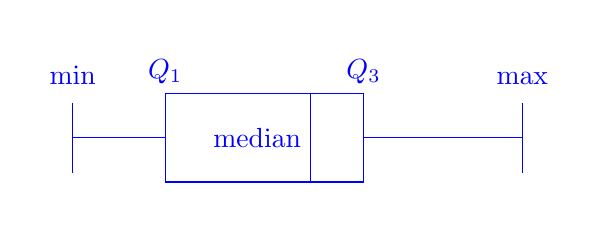
\begin{tikzpicture}
\begin{axis}[
y=1.4cm, 
ymax=2,
ytick=\empty,
xtick=\empty,
axis lines=none
]
\addplot+[
boxplot,
]
table[row sep=\\,y index=0] {
data\\
-2\\ 1\\ 2\\ 1\\ 5\\ 4\\ 10\\
7\\ 10\\ 9\\ 8\\ 9\\ 9\\ 15\\
}
[above]
node at
(boxplot box cs: \boxplotvalue{lower whisker},1)
{min}
node at
(boxplot box cs: \boxplotvalue{lower quartile},1)
{$Q_1$}
node[left] at
(boxplot box cs: \boxplotvalue{median},0.5)
{median}
node at
(boxplot box cs: \boxplotvalue{upper quartile},1)
{$Q_3$}
node at
(boxplot box cs: \boxplotvalue{upper whisker},1)
{max}
;
\end{axis}
\end{tikzpicture}
\end{center}
\end{definition}
\end{frame}

\begin{frame}
\begin{example}
The table lists, in order from lowest to highest, the 50 smart phone speeds, in Mbps.

\vspace{-3mm}
\temporal<2-4>{%
\begin{center}
\begin{tabular}{|rrrrrrrrrr|}\hline
\textcolor{red}{0.8} & 1.4 & 1.8 & 1.9 & 3.2 & 3.6 & 4.5 & 4.5 & 4.6 & 6.2 \\
6.5 & 7.7 & 7.9 & 9.9 & 10.2 & 10.3 & 10.9 & 11.1 & 11.1 & 11.6 \\
11.8 & 12.0 & 13.1 & 13.5 & 13.7 & 14.1 & 14.2 & 14.7 & 15.0 & 15.1 \\
15.5 & 15.8 & 16.0 & 17.5 & 18.2 & 20.2 & 21.1 & 21.5 & 22.2 & 22.4 \\
23.1 & 24.5 & 25.7 & 28.5 & 34.6 & 38.5 & 43.0 & 55.6 & 71.3 & 77.8 \\\hline
\end{tabular}
\end{center}
}{%
\begin{center}
\begin{tabular}{|rrrrrrrrrr|}\hline
\textcolor<1-|handout:0>{blue}{\textcolor<1:handout:1>{red}{0.8}} &
\textcolor<1-|handout:0>{blue}{1.4} &
\textcolor<1-|handout:0>{blue}{1.8} &
\textcolor<1-|handout:0>{blue}{1.9} &
\textcolor<1-|handout:0>{blue}{3.2} &
\textcolor<1-|handout:0>{blue}{3.6} &
\textcolor<1-|handout:0>{blue}{4.5} &
\textcolor<1-|handout:0>{blue}{4.5} &
\textcolor<1-|handout:0>{blue}{4.6} &
\textcolor<1-|handout:0>{blue}{6.2} \\
\textcolor<1-|handout:0>{blue}{6.5} &
\textcolor<1-|handout:0>{blue}{7.7} &
\temporal<2>{\textcolor{blue}{7.9}}{\textcolor{red}{7.9}}{\textcolor{blue}{7.9}} &
\temporal<3|handout:0>{\textcolor{cyan}{9.9}}{\textcolor{blue}{9.9}}{\textcolor{blue}{\textcolor<0:handout:1>{black}{9.9}}} &
\temporal<3|handout:0>{\textcolor{cyan}{10.2}}{\textcolor{blue}{10.2}}{\textcolor{blue}{\textcolor<0:handout:1>{black}{10.2}}} &
\temporal<3|handout:0>{\textcolor{cyan}{10.3}}{\textcolor{blue}{10.3}}{\textcolor{blue}{\textcolor<0:handout:1>{black}{10.3}}} &
\temporal<3|handout:0>{\textcolor{cyan}{10.9}}{\textcolor{blue}{10.9}}{\textcolor{blue}{\textcolor<0:handout:1>{black}{10.9}}} &
\temporal<3|handout:0>{\textcolor{cyan}{11.1}}{\textcolor{blue}{11.1}}{\textcolor{blue}{\textcolor<0:handout:1>{black}{11.1}}} &
\temporal<3|handout:0>{\textcolor{cyan}{11.1}}{\textcolor{blue}{11.1}}{\textcolor{blue}{\textcolor<0:handout:1>{black}{11.1}}} &
\temporal<3|handout:0>{\textcolor{cyan}{11.6}}{\textcolor{blue}{11.6}}{\textcolor{blue}{\textcolor<0:handout:1>{black}{11.6}}} \\
\temporal<3|handout:0>{\textcolor{cyan}{11.8}}{\textcolor{blue}{11.8}}{\textcolor{blue}{\textcolor<0:handout:1>{black}{11.8}}} &
\temporal<3|handout:0>{\textcolor{cyan}{12.0}}{\textcolor{blue}{12.0}}{\textcolor{blue}{\textcolor<0:handout:1>{black}{12.0}}} &
\temporal<3|handout:0>{\textcolor{cyan}{13.1}}{\textcolor{blue}{13.1}}{\textcolor{blue}{\textcolor<0:handout:1>{black}{13.1}}} &
\temporal<3|handout:0>{\textcolor{cyan}{13.5}}{\textcolor{blue}{13.5}}{\textcolor{blue}{\textcolor<0:handout:1>{black}{13.5}}} &
\temporal<3>{\textcolor{cyan}{13.7}}{\textcolor{red}{13.7}}{\textcolor{blue}{13.7}} &
\temporal<3>{\textcolor{cyan}{14.1}}{\textcolor{red}{14.1}}{\textcolor{blue}{14.1}} &
\temporal<4|handout:0>{\textcolor{cyan}{14.2}}{\textcolor{blue}{14.2}}{\textcolor{blue}{\textcolor<0:handout:1>{black}{14.2}}} &
\temporal<4|handout:0>{\textcolor{cyan}{14.7}}{\textcolor{blue}{14.7}}{\textcolor{blue}{\textcolor<0:handout:1>{black}{14.7}}} &
\temporal<4|handout:0>{\textcolor{cyan}{15.0}}{\textcolor{blue}{15.0}}{\textcolor{blue}{\textcolor<0:handout:1>{black}{15.0}}} &
\temporal<4|handout:0>{\textcolor{cyan}{15.1}}{\textcolor{blue}{15.1}}{\textcolor{blue}{\textcolor<0:handout:1>{black}{15.1}}} \\
\temporal<4|handout:0>{\textcolor{cyan}{15.5}}{\textcolor{blue}{15.5}}{\textcolor{blue}{\textcolor<0:handout:1>{black}{15.5}}} &
\temporal<4|handout:0>{\textcolor{cyan}{15.8}}{\textcolor{blue}{15.8}}{\textcolor{blue}{\textcolor<0:handout:1>{black}{15.8}}} &
\temporal<4|handout:0>{\textcolor{cyan}{16.0}}{\textcolor{blue}{16.0}}{\textcolor{blue}{\textcolor<0:handout:1>{black}{16.0}}} &
\temporal<4|handout:0>{\textcolor{cyan}{17.5}}{\textcolor{blue}{17.5}}{\textcolor{blue}{\textcolor<0:handout:1>{black}{17.5}}} &
\temporal<4|handout:0>{\textcolor{cyan}{18.2}}{\textcolor{blue}{18.2}}{\textcolor{blue}{\textcolor<0:handout:1>{black}{18.2}}} &
\temporal<4|handout:0>{\textcolor{cyan}{20.2}}{\textcolor{blue}{20.2}}{\textcolor{blue}{\textcolor<0:handout:1>{black}{20.2}}} &
\temporal<4|handout:0>{\textcolor{cyan}{21.1}}{\textcolor{blue}{21.1}}{\textcolor{blue}{\textcolor<0:handout:1>{black}{21.1}}} &
\temporal<4>{\textcolor{cyan}{21.5}}{\textcolor{red}{21.5}}{\textcolor{blue}{21.5}} &
\textcolor<1-|handout:0>{cyan}{22.2} &
\textcolor<1-|handout:0>{cyan}{22.4} \\
\textcolor<1-|handout:0>{cyan}{23.1} &
\textcolor<1-|handout:0>{cyan}{24.5} &
\textcolor<1-|handout:0>{cyan}{25.7} &
\textcolor<1-|handout:0>{cyan}{28.5} &
\textcolor<1-|handout:0>{cyan}{34.6} &
\textcolor<1-|handout:0>{cyan}{38.5} &
\textcolor<1-|handout:0>{cyan}{43.0} &
\textcolor<1-|handout:0>{cyan}{55.6} &
\textcolor<1-|handout:0>{cyan}{71.3} &
\textcolor<1-|handout:0>{cyan}{\textcolor<0:handout:1>{red}{77.8}} \\\hline
\end{tabular}
\end{center}
}{%
\begin{center}
\begin{tabular}{|rrrrrrrrrr|}\hline
0.8 & 1.4 & 1.8 & 1.9 & 3.2 & 3.6 & 4.5 & 4.5 & 4.6 & 6.2 \\
6.5 & 7.7 & 7.9 & 9.9 & 10.2 & 10.3 & 10.9 & 11.1 & 11.1 & 11.6 \\
11.8 & 12.0 & 13.1 & 13.5 & 13.7 & 14.1 & 14.2 & 14.7 & 15.0 & 15.1 \\
15.5 & 15.8 & 16.0 & 17.5 & 18.2 & 20.2 & 21.1 & 21.5 & 22.2 & 22.4 \\
23.1 & 24.5 & 25.7 & 28.5 & 34.6 & 38.5 & 43.0 & 55.6 & 71.3 & \textcolor<5>{red}{77.8} \\\hline
\end{tabular}
\end{center}
}

\vspace{-1.5mm}
The five number summary is:

\vspace{-3mm}
\begin{center}
minimum=$\textcolor<1>{red}{0.8}$,\pause~$Q_1=\textcolor<2>{red}{7.9}$,\pause~Median=$\textcolor<3>{red}{13.9}$,\pause~$Q_3=\textcolor<4>{red}{21.5}$,\pause~maximum=$\textcolor<5>{red}{77.8}$\pause
\end{center}

\vspace{-2mm}
The box plot is:
\begin{center}
\begin{tikzpicture}
\begin{axis}[
width=\linewidth,
height=5cm,
xlabel={},
ylabel={},
yticklabels={},
axis y line=none,
axis x line=bottom,
y=2cm,
xmin=0,
xmax=80,
]
\addplot+ [
boxplot prepared={
lower whisker=0.8,
lower quartile=7.9,
median=13.9,
upper quartile=21.5,
upper whisker=77.8,
},
]
table [row sep=\\,y index=0] {
data\\
};
\end{axis}
\end{tikzpicture}
\end{center}
\end{example}
\end{frame}

\begin{frame}
\begin{definition}
The \textbf{interquartile range} (\textbf{IQR}) is $Q_3-Q_1$.
\end{definition}\pause

\begin{definition}
A data value is often considered an \textbf{outlier} if
\begin{itemize}
\item  The data value is greater than $Q_3 + 1.5\cdot\textbf{IQR}$.
\item  The data value is less than $Q_1 - 1.5\cdot\textbf{IQR}$.
\end{itemize}
\end{definition}\pause

\begin{block}{Why Care About Outliers?}
Examining data for outliers can help identify:
\begin{itemize}
\item Strong skew in the distribution.\pause
\item Possible data collection or data entry errors.\pause
\item Insights into some interesting property of the data.
\end{itemize}
\end{block}
\end{frame}

\begin{frame}
\begin{example}
The table lists 50 smartphone speeds, in Mbps.
\begin{center}
\begin{tabular}{|rrrrrrrrrr|}\hline
38.5 & \textcolor<11|handout: 1>{red}{55.6} & 22.4 & 14.1 & 23.1 & 24.5 & 6.5 & 21.5 & 25.7 & 14.7 \\
\textcolor<11|handout: 1>{red}{77.8} & \textcolor<11|handout: 1>{red}{71.3} & \textcolor<11|handout: 1>{red}{43.0} & 20.2 & 15.5 & 13.7 & 11.1 & 13.5 & 10.2 & 21.1 \\
15.1 & 14.2 & 4.5 & 7.9 & 9.9 & 10.3 & 6.2 & 17.5 & 22.2 & 13.1 \\
18.2 & 28.5 & 15.8 & 15.0 & 11.1 & 11.8 & 16.0 & 10.9 & 1.8 & 34.6 \\
4.6 & 12.0 & 11.6 & 3.6 & 1.9 & 7.7 & 0.8 & 4.5 & 1.4 & 3.2 \\\hline
\end{tabular}
\end{center}

\vspace{-0.9mm}
Recall that the five number summary is:
\vspace{-2mm}
\begin{center}
minimum=$0.8$, $Q_1=\textcolor<6|handout: 0>{red}{\textcolor<3|handout: 0>{blue}{7.9}}$, Median=$13.9$, $Q_3=\textcolor<9|handout: 0>{red}{\textcolor<3|handout: 0>{red}{21.5}}$, maximum=$77.8$\pause
\end{center}

\vspace{-1.5mm}
The IQR would then be:
\vspace{-2mm}
\begin{equation*}
\text{IQR} = Q_3 - Q_1\pause = \textcolor<3|handout: 0>{red}{21.5} - \textcolor<3|handout: 0>{blue}{7.9}\pause = \textcolor<9|handout: 0>{blue}{\textcolor<6|handout: 0>{blue}{13.6}}
\end{equation*}\pause

\vspace{-7mm}
The limits for outliers would be:
\vspace{-2.5mm}
\begin{equation*}
\begin{aligned}
\text{Lower Limit} &= Q_1 - 1.5 \cdot \text{IQR}\pause = \textcolor<6|handout: 0>{red}{7.9} - 1.5\cdot \textcolor<6|handout: 0>{blue}{13.6}\pause = -12.5 \\\pause
\text{Upper Limit} &= Q_3 + 1.5\cdot \text{IQR}\pause = \textcolor<9|handout: 0>{red}{21.5} + 1.5\cdot \textcolor<9|handout: 0>{blue}{13.6}\pause  = 41.9
\end{aligned}
\end{equation*}\pause

\vspace{-3.5mm}
The outliers are marked in red.
\end{example}
\end{frame}

\begin{frame}
\begin{example}
\texttt{intrest\_rate} has an outlier at $26.3\%$.
\begin{center}
\begin{tikzpicture}
\pgfplotsset{ every non boxed x axis/.append style={x axis line style=-},
     every non boxed y axis/.append style={y axis line style=-}}
\begin{axis}[
width=12cm,
height=4cm,
xlabel={Interest Rate (Rounded to Nearest Percent)},
ylabel={},
yticklabels={},
axis y line=none,
axis x line=bottom,
xticklabel=\pgfmathprintnumber{\tick}\%,
xtick={5,10,...,40},
ymin=0,
ymax=10,
xmin=0,
xmax=40,
scatter/use mapped color={
 %draw=mapped color,
 fill=blue,
},
]
\addplot[domain=0:40]  {1};
\addplot[scatter, only marks, blue, scatter src=y, mark size=2.8pt]
coordinates
{
(11, 1.8)
(11, 2.8)
(11, 3.8)
(11, 4.8)
(11, 5.8)
(10, 1.8)
(10, 2.8)
(10, 3.8)
(10, 4.8)
(10, 5.8)
(10, 6.8)
(10, 7.8)
(10, 8.8)
(9, 1.8)
(9, 2.8)
(9, 3.8)
(9, 4.8)
(9, 5.8)
(17, 1.8)
(17, 2.8)
(17, 3.8)
(6, 1.8)
(6, 2.8)
(6, 3.8)
(8, 1.8)
(8, 2.8)
(8, 3.8)
(8, 4.8)
(13, 1.8)
(13, 2.8)
(13, 3.8)
(5, 1.8)
(5, 2.8)
(5, 3.8)
(7, 1.8)
(7, 2.8)
(7, 3.8)
(7, 4.8)
(7, 5.8)
(18, 1.8)
(18, 2.8)
(19, 1.8)
(14, 1.8)
(20, 1.8)
(15, 1.8)
(12, 1.8)
(16, 1.8)
(21, 1.8)
(25,1.8)
};
\only<1-2|handout: 1>{\addplot[scatter, only marks, red, scatter src=y, mark size=2.8pt, scatter/use mapped color={fill=red,}] coordinates {(26, 1.8)};}
\only<3|handout: 0>{\addplot[scatter, only marks, red, scatter src=y, mark size=2.8pt, scatter/use mapped color={fill=red,}] coordinates {(15, 2.8)};}
\only<4|handout:0>{\addplot[scatter, only marks, red, scatter src=y, mark size=2.8pt, scatter/use mapped color={fill=red,}] coordinates {(35, 1.8)};}
\end{axis}
\end{tikzpicture}
\end{center}
What would happen if this loan had a different interest rate?\pause

\begin{center}
\begin{tabular}{lcccc}
scenario & median & IQR & $\bar{x}$ & $s$ \\\hline
original value of $26.3\%$ & $9.93\%$ & $5.76\%$ & $11.57\%$ & $5.05\%$ \\\pause
move $26.3\%\rightarrow 15\%$ & $9.93\%$ & $5.76\%$ & $11.34\%$ & $4.61\%$ \\\pause
move $26.3\%\rightarrow 35\%$ & $9.93\%$ & $5.76\%$ & $11.74\%$ & $5.68\%$
\end{tabular}
\end{center}
\end{example}
\end{frame}

\begin{frame}
\begin{definition}
A statistic is called \textbf{robust} if extreme observations have little effect on the value.
\end{definition}\pause

\begin{block}{Robustness}
The robust statistics are:
\begin{itemize}
\item The median.
\item The IQR.\@
\end{itemize}\pause

The non-robust statistics are:
\begin{itemize}
\item The mean.
\item The standard deviation.
\end{itemize}
\end{block}
\end{frame}

\begin{frame}
\begin{example}
The distribution of loan amounts in the \texttt{loan50} data set is skewed right, with a few large loans lingering out into the right tail.
\begin{center}
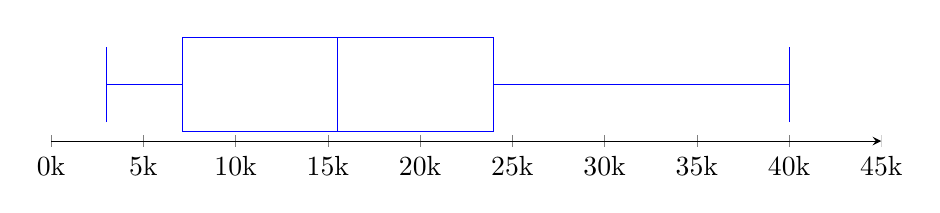
\begin{tikzpicture}
\begin{axis}[
width=\linewidth,
height=2.5cm,
xlabel={},
ylabel={},
yticklabels={},
axis y line=none,
axis x line=bottom,
xticklabel=\pgfmathprintnumber{\tick}k,
scaled x ticks=base 10:-3,
xtick scale label code/.code={},
y=1.5cm,
xmin=0,
xmax=45000,
]
\addplot+ [
boxplot prepared={
lower whisker=3000,
lower quartile=7125,
median=15500,
upper quartile=24000,
upper whisker=40000,
},
]
table [row sep=\\,y index=0] {
data\\
};
\end{axis}
\end{tikzpicture}
\end{center}
\question{If you wanted to understand a typical loan size, should you be more interested in the mean or the median?}\pause
\answer{It depends!}\pause

\vspace{1.5mm}
If we wish to know what a typical loan looks like, the median would probably be more useful. \pause

\vspace{1.5mm}
But, if the goal is something that scales well, such as how much money a bank has to have on hand to cover 1,000 loans, the mean would be more useful.
\end{example}
\end{frame}
\end{document}
